\chapter{Kommunikation}
\section{Architektur}
Man könnte ein IoT System in vier wichtige Gruppen unterteilen: \cite{IoTNetworks}
\begin{itemize}
\item Dinge (things)
\item das lokale Netzwerk
\item das Internet
\item Back-End Services (z.B. Cloud Services)
\end{itemize}
\begin{figure}[H]
\centering
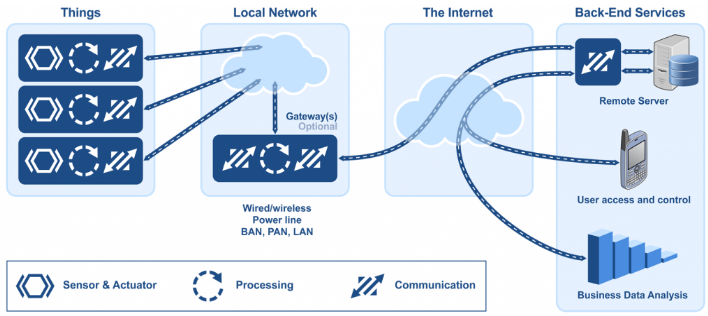
\includegraphics[scale=0.8]{../02_Analyse/images/iot_system_overview_by_micrium.png}
\caption{IoT Systemübersicht\cite{IoTOverview}}
\end{figure}
Grundsätzlich scheint die Architektur vertraut. Smart Objects kommunizieren über ein lokales Netzwerk mit Diensten im Internet.

Bisher konnten Geräte wie Laptops, PCs und Smartphones beinahe einheitlich mit dem Internet verbunden werden; entweder verkabelt über Ethernet oder drahtlos über ein lokales WLAN oder mobile Netze wie UMTS und LTE. Die Endgeräte verfügten jeweils über viel Rechenleistung, Speicher und ein leistungsfähiges Betriebssystem mit einem vollständig implementierten TCP/IP Stack. 

In einem IoT System muss man von einer grossen Anzahl an Geräten mit Sensoren ausgehen. Manchmal verfügen diese Geräte über eine extrem niedrige Bandbreite, wenig Speicher und Rechenleistung \cite{CiscoIoTArchitecture}.

Die Kommunikation erfolgt oft nicht vertikal der Architektur, sondern auch horizontal auf derselben Ebene. Sensordevices können beispielsweise miteinander kommunizieren oder Cloud Services Daten der Sensoren untereinander austauschen.
\subsection{Wireless Sensor Netzwerke}
Bei einer Vielzahl von verbundenen Sensoren, welche über einen grossen Bereich verstreut sind, bietet sich ein Wireless Sensor Network (WSN) an. In einem WSN werden die Sensoren nicht direkt mit dem Internet verbunden. Die Daten werden drahtlos von Teilnehmer zu Teilnehmer versendet. Muss ein Datenpaket in ein entferntes Netzwerk wie das Internet, so wird ein Gateway oder Edge Node benötigt.
\begin{figure}[H]
\centering
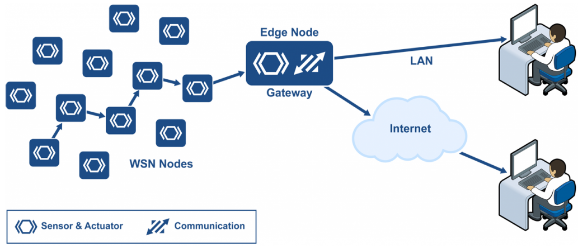
\includegraphics[scale=0.8]{../02_Analyse/images/iot_wsn_lan_overview_by_micrium.png}
\caption{IoT WSN\cite{IoTWSN}}
\end{figure}
WSN Nodes sind typischerweise günstig im Einkauf. Sie können mit sehr wenig Leistung betrieben werden, dies ermöglicht den Batteriebetrieb. Durch diese Eigenschaften können WSN Nodes einfach, schnell und in sehr grosser Anzahl bereitgestellt werden. 

\section{Kommunikationsmodelle}
Internet of Things verbindet Objekte aus der realen Welt miteinander. Um Objekte aus der Realität in die virtuelle Welt zu transformieren, werden Sensoren verwendet. Es gilt nun, diese Sensoren mit dem Internet zu verbinden.

Um unterschiedliche Bedürfnisse abzudecken, sind verschiedene Arten der Kommunikation entstanden. Die mit Sensoren ausgestatteten Geräte können sich in ihrer Weise, mit dem Internet zu kommunizieren stark unterscheiden.

\subsection{Device-to-Device}
Beim Device-to-Device Kommunikationsmodell kommunizieren mehrere Teilnehmer direkt miteinander (Peer-to-Peer). In diesem Szenario kommunizieren unterschiedliche Glühbirnen drahtlos mit einem Lichtschalter. Denkbar wären sämtliche Anwendungsgebiete aus dem \glqq Smart Home\grqq -Bereich. Kommunikation mit dem Internet ist nicht zwingend notwendig. Eine grosse Herausforderung besteht darin, dass mehrere Teilnehmer unterschiedlicher Hersteller miteinander interagieren können. Dazu müssen die Teilnehmer denselben Protokoll-Stack implementieren. 
\begin{figure}[H]
\centering
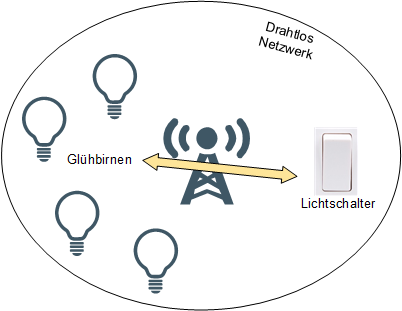
\includegraphics[scale=0.8]{../02_Analyse/images/device-to-device.png}
\caption{Device-to-Device Kommunikation}
\end{figure}
\subsection{Device-to-Cloud}
Die Gerätehersteller bieten für ihre End-User Cloud-Dienste im Internet an. Die Sensorgeräte kommunizieren direkt End-to-End über TCP/IP mit dem jeweiligen Cloud-Dienst. Die Benutzer können über eine Mobile App oder eine Webseite auf die jeweiligen Sensordaten zugreifen. Häufig wird aufgrund proprietärer Kommunikationsprotokolle ein Vendor-lock-in betrieben. Dies erschwert die Interoperabilität von Sensoren unterschiedlicher Hersteller \cite{RoseEldridgeChapin15}.
\begin{figure}[H]
\centering
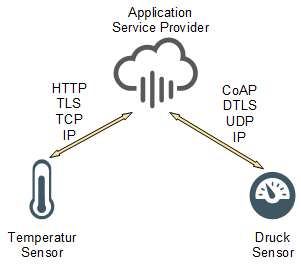
\includegraphics[scale=0.8]{../02_Analyse/images/device-to-cloud.png}
\caption{Device-to-Cloud Kommunikation}
\end{figure}
\subsection{Device-to-Gateway}
Anstatt einer Ende-zu-Ende Kommunikation zwischen Sensoren und Servern wird in diesem Modell ein Gateway zwischen diesen Komponenten eingesetzt. Sensoren kommunizieren somit nicht direkt mit einem Server. Auf diese Art und Weise können eine grosse Anzahl Sensoren mit Internetdiensten verbunden werden ohne dass die Sensoren selbst über einen direkten Internetzugriff verfügen. Der Gateway muss somit über eine Schnittstelle verfügen, damit Dienste im Internet indirekt mit den Sensoren kommunizieren können. Aus Sicht des Diensts ist es irrelevant, wie der Gateway mit den Sensoren kommuniziert.
\begin{figure}[H]
\centering
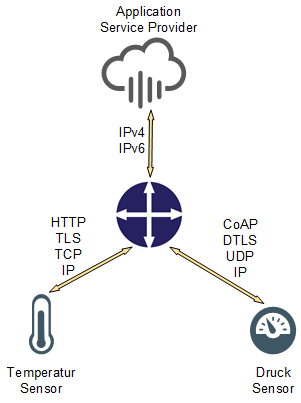
\includegraphics[scale=0.8]{../02_Analyse/images/device-to-gateway.png}
\caption{Device-to-Gateway Kommunikation}
\end{figure}
\subsection{Back-End Data-Sharing}
Sobald sich die Sensordaten auf einem Server befinden, können diese auf bekannte Weise anderen zur Verfügung gestellt werden. Beispielsweise könnte man den Zustand eines Sensors als JSON Objekt über eine REST-Schnittstelle abfragen. Ein weiterer Serviceprovider muss somit nicht mehr direkt mit den Sensoren kommunizieren. Da Sensordevices oft über limitierte Möglichkeiten verfügen, grössere Datenmengen bereitzustellen, verringert man mit dieser Art der Kommunikation die Anzahl Abfragen auf den Sensordevices. 
\begin{figure}[H]
\centering
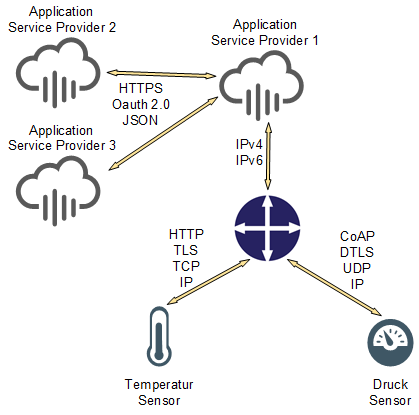
\includegraphics[scale=0.8]{../02_Analyse/images/backend-data-sharing.png}
\caption{Backend-Data-Sharing Kommunikation}
\end{figure}

\newpage

\section{IoT Kommunikationsprotokolle}
Seit der Entstehung des Internets werden für unterschiedliche Aufgaben Kommunikationsprotokolle entwickelt. Eine grosse Herausforderung war stets die Interoperabilität zwischen Geräten unterschiedlicher Hersteller. Standardisierungsgremien wie die International Standards Organization (ISO) und die Internet Engineering Task Force (IETF) haben in den vergangenen Jahrzehnten Richtlinien und Standardisierung von Kommunikationsprotokollen veröffentlicht. 

Mit zunehmender Popularität des Internets der Dinge sind eine unüberschaubare Menge an proprietären und offenen Kommunikationsprotokollen entstanden. In der Geschichte des Internets hat sich gezeigt, dass sich langfristig nur offene Protokolle durchsetzen werden \cite{Obermaier14}, proprietäre Protokolle hingegen werden aufgrund der fehlenden Interoperabilität niemals eine breite Verwendung finden.
\subsection{Anforderungen}
Bereits heute zeichnen sich die populärsten IoT Kommunikationsprotokolle ab. Um zu verstehen weshalb-, und vor allem in welchen Szenarien welches Protokoll eingesetzt wird respektive werden sollte, muss man sich mit den unterschiedlichen Anforderungen vertraut machen.

Die typischen bekannten Fragen nach der Verbreitung/Unterstützung und Skalierbarkeit stellen sich auch hier. Ebenfalls muss auf die mutmassliche Datenmenge geachtet werden. So dürfte eine vergleichsweise hohe Datenmenge für Geräte, welche über einen direkten, verkabelten Internetzugang verfügen, kein Problem darstellen, während Geräte in einem Mesh-betriebenen WSN wohl über deutlich weniger Bandbreite verfügen dürften.

Weitere Anforderungen wären Realtime Kommunikation, Stromverbrauch, Sicherheit und Network Address Translation (NAT) \cite{Obermaier15}.
\subsection{Request/Response}
Request/Response ist das wohl bekannteste Pattern. Ein Client fordert mittels eines Requests eine Response von einem Service an. Der Service hört auf einkommende Requests, verarbeitet diese und antwortet (Response) den aufrufenden Clients. Request/Response Kommunikation skaliert schlecht, deshalb sollte beim Versenden einer Meldung an viele Teilnehmer auf ein anderes Pattern zurückgegriffen werden. 
\begin{figure}[H]
\centering
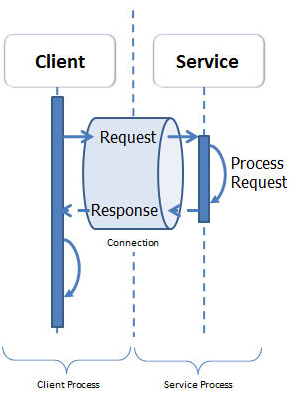
\includegraphics[scale=0.8]{../02_Analyse/images/request-response.png}
\caption{Request/Response Kommunikation \cite{ReqRes}}
\end{figure}
\subsubsection{HTTP}
In den 1990er Jahren wurde HTTP verwendet um statische HTML-Dokumente übers Internet abzurufen. Bis heute hat sich die grundsätzliche Funktion von HTTP nicht verändert. HTTP bietet über seine Methoden ein umfangreiches Interface für die Request/Response Kommunikation zwischen Clients und Servern über das Internet. 

Aufgrund seiner hohen Verbreitung, Standardisierung und Unterstützung ist HTTP auch im IoT Umfeld beliebt. Für fast jede Programmiersprache und Laufzeitumgebung existieren Libraries, was das Entwickeln sehr angenehm macht. HTTP eignet sich jedoch nicht für alle Anwendungsfälle im IoT Bereich. Für jeden Request wird der gesamte HTTP (und darunterliegende) Header benötigt. Zusätzlich ist das Protokoll textbasiert, was mit dem zusätzlichen, grossen Overhead eine erhebliche Datenmenge bedeuten könnte. Für Endgeräte an Mobilen Netzwerken könnte dies ungeeignet sein \cite{Obermaier15}.

In der Version 1, respektive 1.1 gibt es mit HTTP keine Möglichkeit, echte Push-Meldungen zu versenden. Bei Push-Meldungen sendet der Server eine Response (besser: Nachricht) an den Client ohne vorgängigen Request. In der Version 2 von HTTP sind echte Push-Meldungen vorgesehen, jedoch gibt es wenige Implementation und Erfahrungswerte damit.
\subsubsection{CoAP}
Das Constrained Application Protocol (CoAP) implementiert wie HTTP das Request/Response Pattern \cite{Obermaier15}. Mit CoAP existiert ein massgeschneidertes IoT-Protokoll, welches nach dem REST Paradigma konzipiert wurde. HTTP ist schwergewichtig, hat einen grossen Overhead und generiert damit hohe Datenmengen. Ausserdem ist vor jeder Session den für TCP benötigten 3-Way Handshake nötig. 
 
CoAP wurde entwickelt, um diesen Schwächen von HTTP entgegenzuwirken. Bei sogenannten Low-Power and Lossy Networks (LLN's) sind die Nodes im Vergleich zu herkömmlichen Computersystemen sehr eingeschränkt, was die Verwendung von HTTP schwierig gestaltet. CoAP bietet grundsätzlich folgende Features:\cite{RFC7252}
\begin{itemize}
\item Request/Response Kommunikation zwischen Endpoints	
\item Discovery von Services und Ressourcen
\item URI's und Media Types
\item Kompatibilität mit HTTP
\item Multicast Support
\item sehr kleiner Overhead (Header von 4 Byte)
\item implementiert das Observer Design Pattern
\item UDP als Transportprotokoll
\item Asynchroner Nachrichtenaustausch
\end{itemize}
 
CoAP kann Peer-to-Peer zwischen Devices eingesetzt werden, aber auch zwischen Device und Service oder zwischen Device und einem Proxy.
\begin{figure}[H]
\centering
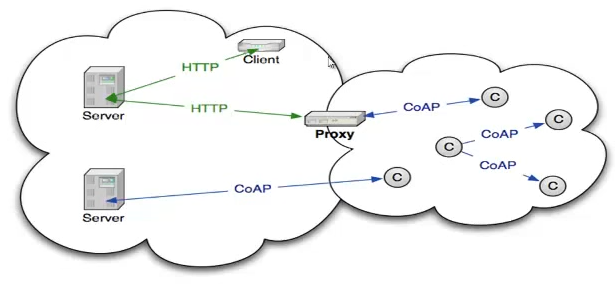
\includegraphics[scale=0.8]{../02_Analyse/images/coap_architecture.png}
\caption{CoAP Architektur \cite{Shelby14}}
\end{figure}
  
Durch die massgeschneiderten Features für IoT wird CoAP hauptsächlich in WSN's eingesetzt \cite{Obermaier15}. 

\subsection{Publish/Subscribe}
Beim Publish/Subscribe Pattern gibt es einen Sender (Publisher) und einen Empfänger (Subscriber). Der Empfänger hört auf gewisse Themen (Topics). Dies kann nur ein Thema sein oder auch viele Verschiedene. Der Sender kategorisiert seine Nachrichten in Themen und sendet diese zu den jeweiligen Empfänger. Der Sender und der Empfänger wissen aber nichts voneinander. Sie senden oder hören nur im Netzwerk, ob eine für sie interessante Nachricht angekommen ist. Durch die einfache Verknüpfung von Publisher und Subscriber, eignet sich dieses Verfahren sehr gut im IoT-Bereich. Die Sensoren sind die Publisher, sie liefern zum Beispiel Temperaturdaten in die richtige Kategorie. Alle Server/Clouddienste, welche sich für Temperaturdaten interessieren, können auf diese Kategorie hören. Durch die einfache Handhabung skaliert dieses Pattern sehr gut.

In der folgenden Grafik sieht man das Publish and Subscribe Pattern. Der Publisher hat eine ''Address Changed'' Message in den Channel geschickt. Nun erhalten alle Subscriber, welche dem Channel folgen, diese Nachricht und verarbeiten sie.

\begin{figure}[H]
\centering
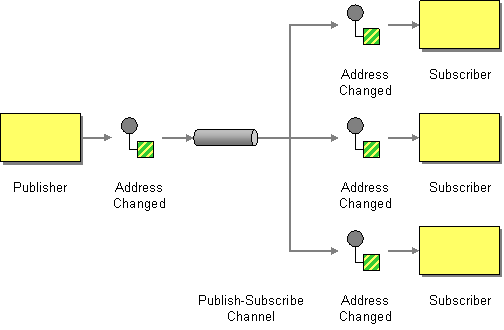
\includegraphics[scale=0.65]{../02_Analyse/images/publishsubscribe.png}
\caption{Publish and Subscribe Pattern\cite{PublishSubscribePattern}}
\end{figure}
\subsubsection{MQTT}
MQTT (Message Queue Telemetry Transport) ist ein von IBM entwickeltes Protokoll. Es ist ein speziell für IoT entwickeltes Protokoll um Machine-to-Machine Kommunikation herzustellen. Bei dem Protokoll wurde speziell auch ein schlankes Design geachtet. So ist die kleinst mögliche Nachricht gerade mal 2 Byte gross. 

Der Hauptverwendungszweck von MQTT ist vor allem der Austausch von Daten zwischen Geräten und Server (D2S).\cite{ProtPubSub} Da das Protokoll für die D2D Konnektivität entwickelt wurde, wird es auch in diesem Bereich eingesetzt. Das heisst die Vorteile liegen in Netzen mit vielen kleinen Geräten, welche wenig Kommunizieren und sich als Kollektion sehen.\cite{ProtPubSubReason}

Bei MQTT wird ein Broker verwendet. Der Sensor ''published'' seine Daten mit einem Topic und den Daten an den Broker. Dieser sendet die Nachricht an alle, welche sich auf das gewünschte Topic Subscribed haben. Durch das schlanke Design, gibt es natürlich auch Nachteile. Aber bei kleinen und einfachen Systemen ist MQTT ein beliebtes Protokoll.
\subsubsection{AMQP}
AMQP (Advanced Message Queuing Protocol) ist ein bekanntes und viel eingesetztes Protokoll. Das binäre Netzwerkprotokoll wird von vielen grossen Firmen\cite{ProtPubSubReason} entwickelt, wie zum Beispiel Microsoft oder auch Cisco. Momentan ist die Version 1.0 seit 2010 als aktuellen Standard im Einsatz.

AMQP wird durch sein Queuing Design im Server zu Server Bereich eingesetzt (S2S).\cite{ProtPubSub} Daher ist es in Bereichen einzusetzen, in der die Geschwindigkeit und der Prozessor nicht relevant sind. Zusätzlich wird es in Bereichen eingesetzt, in dem eine Nachricht nur von A nach B gesendet werden soll und man keine Nachricht verlieren möchte.

Die Sensoren senden die Nachrichten an einen Message Broker, welcher die Nachricht in die richtige Queue schiebt. Nun können sich die Dienste an der Queue anmelden und die Nachrichten konsumieren. Dabei gibt es die Möglichkeit Topics zu setzen, um Kategorien einzuführen. Es können jeder Nachricht auch noch Attribute hinzugefügt werden, wie zum Beispiel Name oder Durability. Durch den grossen Funktionsumfang des Protokolls ist es natürlich auch schwieriger einzurichten und die minimale Paketgrösse wächst damit auch. Die kleinstmögliche Paketgrösse ist 60 Byte.
\subsubsection{XMPP}
XMPP (Extensible Messaging and Presence Protocol) wurde speziell für das Internet der Dinge erweitert, um den Anforderungen gerecht zu werden. XMPP gibt es schon seit mehreren Jahren und wurde in vielen Chatprogrammen eingesetzt. Auch heute findet man das Protokoll beim Facebook-Messenger wieder. Mit der IoT-Erweiterung/Anpassung will man nun nicht mehr Menschen miteinander verknüpfen, sondern Dinge. 

XMPP ist das beste Protokoll um Geräte mit Menschen zu verbinden. Dies ist eine Spezialform des Geräte zu Server Pattern (D2S). \cite{ProtPubSub} XMPP sollte dann verwendet werden, wenn die Geschwindigkeit und der Prozessor nicht wichtig sind, wenn das Gerät immer verbunden sein soll und wenn nur wenige Konnektivitätspunke in einem grossen Bereich vorhanden sind.\cite{ProtPubSubReason}

Bei XMPP wird kein Broker, sondern ein zentraler Server verwendet. Dieser soll allerlei verschiedene Geräte miteinander verbinden. Dieses Protokoll wird häufig für das Remote Management von Konsumergeräten verwendet.

\newpage

\section{LwM2M - Lightweight M2M}
\subsection{Einführung}
LwM2M ist ein speziell für IoT entwickeltes Management- und Messaging-Protokoll. Wie es der Name schon verrät, handelt es sich um ein M2M - Machine-to-Machine Protokoll. Bei LwM2M wird ein Client-Server-Modell umgesetzt. Dabei werden alle Daten per Request angefragt und als Response beantwortet.

Entwickelt und standardisiert wurde dieses durch die Open Mobile Alliance, kurz OMA. Die Oma ist ein Verbund aus Firmen, welche in der Mobilfunksparte tätig sind, wie zum Beispiel Nokia, Motorola oder auch viele grosse Mobilfunkprovider. 

\subsection{Protocol Stack}

LwM2m ist ein Applikationslayer Protokoll und hat als Basis das CoAP Protokoll. Alle LwM2M Befehle werden umgewandelt, damit diese über CoAP zum Geräte gesendet werden. Dabei werden nicht alle Features von CoAP eingesetzt und unterstützt. CoAP ist wie auch LwM2M speziell für M2M (Maschine-to-Machine) Applikationen entwickelt worden.

Unterhalb von CoAP gibt es drei Varianten, die am gebräuchlichsten sind. UDP, UDP mit DTLS und SMS. Verwendet man nur UDP wird keine Verschlüsselung verwendet. Alle Daten werden in Klartext übertragen. Um eine sichere Verbindung herzustellen muss DTLS eingerichtet werden. Zusätzlich gibt es noch die Möglichkeit SMS. Diese ist speziell für Geräte ohne Internetanschluss gedacht. Alle Anfragen werden in ein SMS gepackt und so über das Telekommunikationsnetz übertragen.

Unterhalb der Verbindungsschicht können wieder viele verschiedene Technologien eingesetzt werden. Dies ist unter anderem IPv4, IPv6, 6LoWPAN oder auch ZigBee IP. 

Mit all diesen Möglichkeiten bietet LwM2M eine grosse Abdeckung an Technologien und kann vielseitig eingesetzt werden. 
\begin{figure}[H]
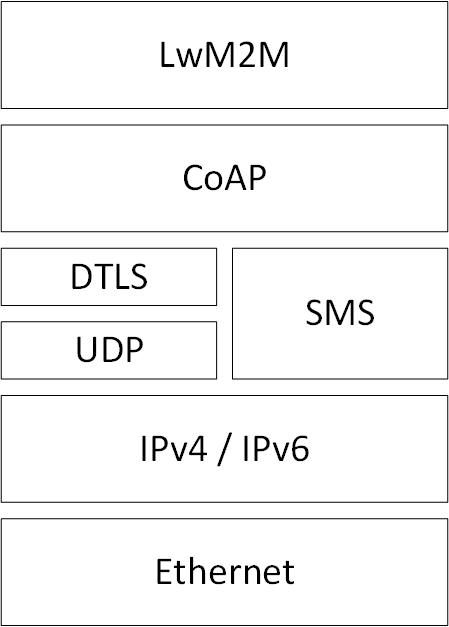
\includegraphics[scale=0.3]{images/lwm2m/stack.png}
\caption{LwM2M Stack}
\end{figure}

\newpage

\subsection{Client-Server Model}
\begin{figure}[H]
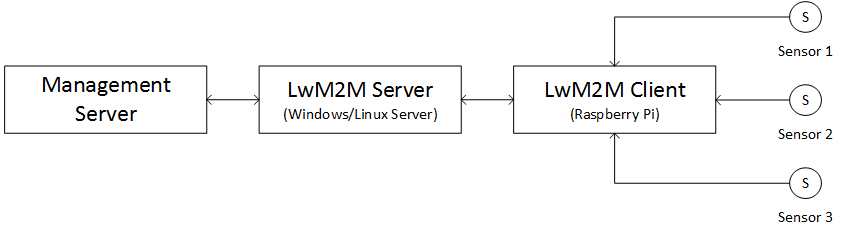
\includegraphics[scale=0.5]{images/lwm2m/server_client_model.png}
\caption{Client-Server-Model}
\end{figure}
Die drei zentralen Bestandteil des Protokolls sind der Bootstrap-Server, der LwM2M-Server und der LwM2M-Client. Der Bootstrap-Server ist für den Erstkontakt sowie die Erstkonfiguration zuständig. Die restliche Kommunikation läuft zwischen dem LwM2M-Server und dem LwM2M-Client. Ohne einen Bootstrap-Server kommunizieren die Geräte direkt mit dem LwM2M-Server.
\subsubsection{Client}
Der Client kann viele verschiedene Formen annehmen. Ein Beispiel wäre eine Linux Installation auf einem Raspberry Pi, welche einen Java LwM2M Client gestartet hat. An dem Raspberry Pi kann man nun mehrere Sensoren, wie Temperatur, Druck, etc. anschliessen und diese über den Client steuern. Es kann sich aber auch nur um einen kleinen Chip mit Sensor handeln, welcher ein C LwM2M Client beinhaltet. Client Umsetzungen gibt es dabei in den Programmiersprachen C und Java.
\subsubsection{Server}
Die Serverumsetzung ist sehr ähnlich wie die Clientumsetzung. Es wird auf einem Server eine Serverinstanz gestartet und diese wartet auf Clients, welche sich Registrieren möchten. Da die Serverimplementierung, wie auch der Client in C und Java verfügbar ist, gibt es viele Möglichkeiten den Server zu deployen. So kann er auf einer Windows- sowie auch unter Linux gestartet werden. Der Server hört dann auf dem CoAP Port auf die Anfragen.
\subsubsection{Management Server}
Der Management Server klinkt sich nun beim LwM2M Server ein. Dieser Server kann direkt oder über ein Web API angesprochen werden. Je nach Implementierung gibt es beide Varianten. So könnte man mehrere Serverinstanzen zu einem Management Server hinzufügen, um alles zentral Verwalten zu können. Möchte man nun ein Gerät managen, schickt man einen Befehl an den zuständigen LwM2M Server und dieser leitet den Befehl nun an das Device weiter. Die Antwort wird danach bis zum Management Server zurückgegeben und ausgewertet. 
\subsubsection{Bootstrap-Server}
Um ein ''factory bootstrap'' zu vermeiden, hat LwM2M einen Bootstrap-Server. Dieser ist für die Erstkonfiguration Zuständig und macht die Devices variabler einsetzbar. Bootstraping wird im Kapitel Features und Funktionen genauer beschrieben.

\newpage

\subsection{Object Model}
Eine klare Stärke des LwM2M-Protokolls sind die Object Models. Durch die Object Models werden alle Informationen eines Devices in einem strukturierten Model abgelegt, damit ein geregelter Zugriff auf alle Daten entsteht. Es wird zwischen Object, Instance und Ressource unterschieden. Eine Ressource ist zum Beispiel der Temperaturwert eines Temperatursensors. Eine zusätzliche Ressource könnte die dazugehörige Temperatureinheit sein. Mehrere solche Ressourcen werden zu einem Object Model zusammengefasst. Ein Device kann aber auch mehrere Temperatursensoren besitzen und hat so mehrere Instanzen des gleichen Objects.

Um nun die Information zugreifbar zu machen, bekommt sie eine URL mit den drei oben beschriebenen angaben. Diese kann wie folgt aussehen.
%TODO Bild einfügen
\begin{figure}[H]
%\includegraphics[scale=0.5]{}
\caption{Object Model URL}
\end{figure}
\subsubsection{Aufbau}
\subsubsection{Object}
Jedes Object besitzt eine eindeutige Identifikationsnummer. Diese geht von 0-32768 und ist folgendermassen verteilt:
\begin{itemize}
\item 0-1023: OMA-Label
\item 1024-2047: Reserviert für zukünftige Benutzung
\item 2048-10240: Registrierungen der Partnerfirmen
\item 10241-32768: Individuelle Registrierungen durch Firmen oder Personen
\end{itemize}
Wenn man ein neues Model erstellen möchte, geht man auf die OMA-Seite und erfasst dieses im ''LWM2M Management Object Editor''. Pro neuem Modell muss man eine Object ID, Namen, ObjectVersion, LWM2MVersion, Object URN, Instances und Mandatory festlegen. Mit Instances gibt man an, ob ein Object pro Device mehrmals vorhanden sein darf.
\subsubsection{Instances}
Wenn ein Object mehrmals vorhanden sein kann, wie zum Beispiel ein Temperaturobjekt, gibt es die Möglichkeit der Multiinstanz. Der mittlere Teil der URL nimmt dadurch nicht nur den Wert 0 an, sondern eine eindeutige ID pro Instanz.

\subsubsection{Ressource}
Dem Object werden zum Schluss noch die Ressourcen hinzugefügt. Diese besitzen auch eine eindeutige Identifikationsnummer von 0 bis 32768. Hier gibt es folgende Unterteilung:
\begin{itemize}
\item 0-2047: Common Ressources
\item 2048-26240: Reusable Ressources
\item 26241-32768: Private Ressources
\end{itemize}
Jede Ressource hat vordefinierte Felder. Dazu gehören Name, Operations, MultipleInstances, Mandatory, Type, RangeEnumeration, Units und Description. Durch all diese Felder kann eine Ressource sehr genau beschrieben werden. Nicht alle Felder sind Pflicht, aber wichtig sind vorallem ID, Name und Operations und Type. Durch die Operations gibt man an, was mit dieser Ressource genau gemacht werden kann. Hier kann man zwischen Read, Write, Read-Write und Execute wählen.	Mit dem Type Feld gibt man den Type Informationstyp an, wie zum Beispiel String, Float oder Date.


Durch all diese Standardisierten Objekte und Ressourcen kann man jede Information eines Gerätes beschreiben und es entstehen keine Kompatibilitätsprobleme.
\subsubsection{Beispiel XML}
Hier sieht man ein Beispiel von dem Object Model ''Device'' mit der Ressource ''0 - Manufacturer''. Das Object Model besitzt aber noch weitere Ressourcen, die andere Informationen eines Devices definieren.
\begin{lstlisting}[%
language=xml]
<LWM2M>
	<Object">
		<Name>Device</Name>
		<Description1><![CDATA[ This LWM2M Object ... ]]></Description1>
		<ObjectID>3</ObjectID>
		<ObjectURN>TBD</ObjectURN>
		<MultipleInstances>Single</MultipleInstances>
		<Mandatory>Mandatory</Mandatory>
		<Resources>
			<Item ID="0">
				<Name>Manufacturer</Name>
				<Operations>R</Operations>
				<MultipleInstances>Single</MultipleInstances>
				<Mandatory>Optional</Mandatory>
				<Type>String</Type>
				<RangeEnumeration />
				<Units/>
				<Description><![CDATA[ Human rea... ]]</Description>
			</Item>
			<Item>...</Item>
		</Resources>
	</Object>
</LWM2M>
\end{lstlisting}

\subsubsection{Beispiel Client}
Hier sieht man nun ein Beispielclient. Dies könnte eine kleine LED-Lampe sein, welche jedes LED separat steuern lässt. Dazu wurden die Objeke 3 und 3311 verwendet, welche bereits vorgefertigt bereitstehen. Da es mehrere LEDs gibt, werden auch mehrere Light Control Instanzen benötigt. Jede Instanz steuert so eine einzelne LED.
Neben diesen drei Objekten könnten noch weitere vorhanden sein, wie zum Beispiel Firmware oder andere Sensorobjekte.
\begin{figure}[H]
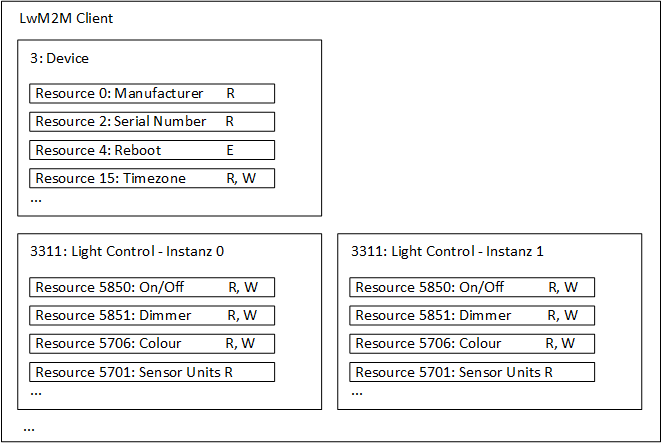
\includegraphics[scale=0.65]{images/lwm2m/lwm2m_client.png}
\caption{LwM2M Stack}
\end{figure}

\newpage

\subsection{Features und Funktionen}
LwM2M bietet vier Funktionen, um mit einem Device zu kommunizieren oder diesen zu konfigurieren. Bootstraping, Registration, Object / Ressource Access und Reporting. Es müssen aber nicht immer alle Funktionen eingesetzt werden. So kann auf Bootstraping und Reporting verzichtet werden, wenn man jedes Device von Hand vorkonfiguriert.
\subsubsection{Bootstrapping - Allgemein}
Wie oben bereits erwähnt, ist das ''factory bootstraping'' möglichst zu vermeiden. Durch die statisch hinterlegten Keys und Server-URLs muss man bei jeder Anpassung der Daten physischen Zugriff auf das Device haben. Dies ist ein Ansatz, der vielleicht bei normalen Computern noch funktioniert hat, aber dies funktioniert bei IoT-Geräten selten gut. Daher hat das LwM2M-Protokoll einen Bootstrap-Vorgang definiert.


Der Hersteller muss für das Bootstraping jedem Gerät ein Endpointname, sowie eine Bootstrap-URL hinterlegen. Alle anderen Informationen, werden beim Starten vom Bootstrap-Server geholt.
Wichtige Einstellungen die der Bootstrap-Server verteilen kann sind unter anderen\cite{BootstrapFeatures}:
\begin{itemize}
\item Keys  und Zertifikate für DTLS
\item Server URL
\item SMS Security Parameter
\item Kommunikationsparameter
\item Access Control Lists
\end{itemize}
Durch den Einsatz von Bootstraping nimmt man sich viel Managementarbeit ab und hat ein einheitlicheres und besser verwaltetes Netzwerk von LwM2M-Server und Client.
\subsubsection{Bootstrapping - Ablauf}
Sobald ein Device gestartet wird, überprüft es seine Einstellungen. Es gibt zwei Zeitpunkte, an denen der Device einen Bootstrap-Server kontaktiert. Der erste ist, sobald der Device nur Bootstrap-Server Daten besitzt und keine LwM2M-Server Daten hinterlegt hat. Die zweite Möglichkeit ist, wenn der L2M2M-Server keine Antwort mehr gibt oder Authentifikation fehlgeschlagen meldet. Sobald dies geschieht, meldet sich der Device wieder beim Bootstrap-Server, um eine neue konfiguration zu erhalten.

In der folgenden Grafik sieht man den Ablauf des Bootstrapings.
\begin{figure}[H]
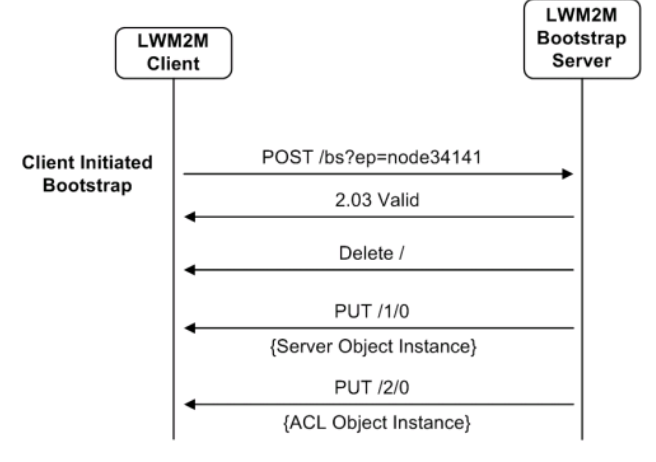
\includegraphics[scale=0.5]{images/lwm2m/bootstrap_diagram.png}
\caption{LwM2M Bootstraping\cite{LwM2MInterfaces}}
\end{figure}
Als ersten Schritt sendet der Device eine Anfrage an den Bootstrap-Server. In dieser Anfrage gibt der Client sein Endpointname an. Durch diesen Endpointname weiss der Bootstrap-Server, welche Konfiguration für dieses Gerät vorgesehen ist. Der Server antwortet mit ''Valid''. Durch einen Delete Befehl auf die Root-URL löscht es die alten Konfigurationen. Danach werden durch einzelne PUTs alle wichtigen Daten auf das Gerät geschrieben.

Wenn der Server eine neue Konfiguration, wie zum Beispiel neues Schlüsselmaterial, verteilen möchte, löscht der LwM2M-Server durch einen Delete wieder die Root-URL auf dem Client. Dadurch meldet sich der Client wieder beim Bootstrap-Server, um die neuen Daten zu erhalten. Dies nennt man den  Server imitierte Bootstrap-Vorgang.

\subsubsection{Registration - Allgemein}
Wenn ein Client einen gültigen und erreichbaren LwM2M-Server hinterlegt hat, beginnt die Registrierungsphase. Bei der Registrierung wird dem Server bekanntgeben, welche Funktionen und Informationen der Client besitzt. Dies beinhaltet die Object Model URLs, Registrierungszeitpunkt, IP-Adresse, Port und noch weitere Angaben, die der Server von jedem Client benötigt. All diese Angaben werden vom Client immer wieder aktualisiert und an den Server gesendet. Dies geschieht meistens mehrmals pro Minute.

\subsubsection{Registration - Ablauf}
\begin{figure}[H]
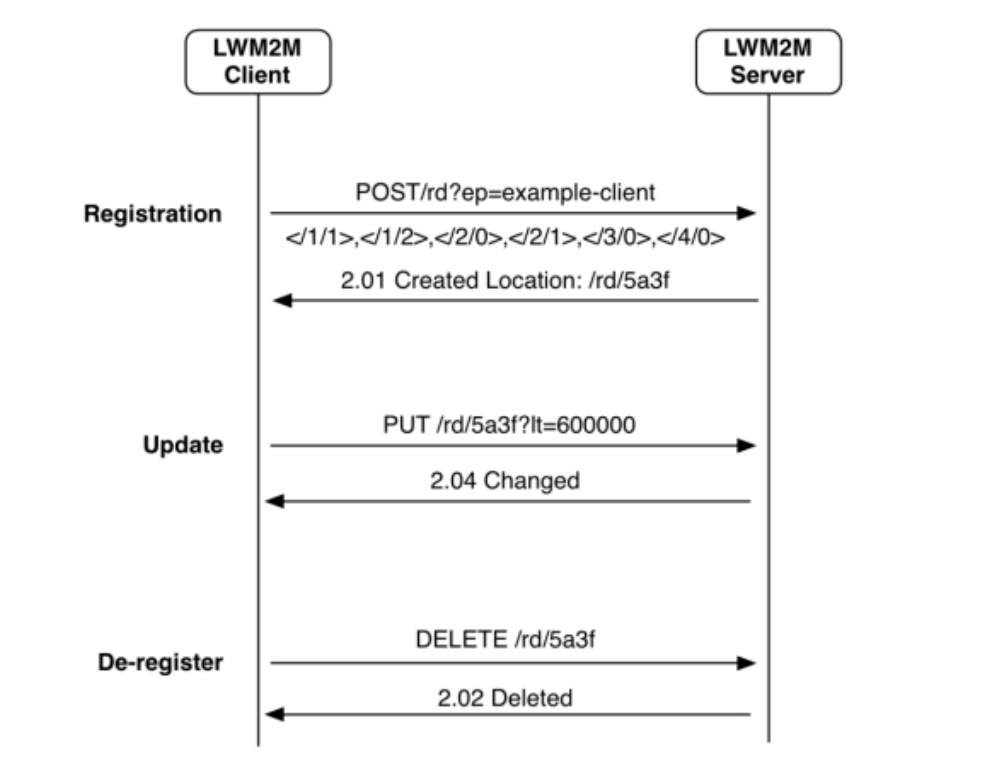
\includegraphics[scale=0.4]{images/lwm2m/registration_diagram.png}
\caption{LwM2M Registration\cite{LwM2MInterfaces}}
\end{figure}
Die Registrierung wird immer von einem Client aus gestartet. Dieser sendet seinem hinterlegtem LwM2M-Server einen POST mit all den relevanten Daten. Sobald diese gesendet wurden, wartet der Client auf eine Antwort. Der Server überprüft nun diese Daten und checkt auch gleichzeitig, ob der Client sich richtig authentifiziert hat. Wenn alle Daten passen, legt der Server eine Registrierung an und sendet dem Client die URL zu dieser Ressource. Der Client kann nun alle weiteren Daten an diese URL senden.

Nach einer gewissen Zeit meldet der Client ein Update an den Server. Durch einen PUT auf die für ihn hinterlegte URL kann er die angepassten Daten an den Server senden. Dieser antwortet mit ''Changed'', falls alles in Ordnung ist.

Wird ein Client heruntergefahren deregistriert sich dieser automatisch bei seinem Server. Dazu sendet der Client ein Delete auf seine Ressource auf dem Server und erhält ''Deleted'' als Antwort. 

\newpage

\subsubsection{Object / Ressource Access - Allgemein}
Nach dem Registrieren kann der Server auf alle für ihn freigegebenen Daten zugreifen. Dies geschieht über drei definierten Anfragen Read, Write und Execute. Um neue Daten auf den Client zu senden, erlauben die Write und Execute Anfragen zusätzliche Daten. All diese Anfragen an den Client werden vom LwM2M-Server in ein CoAP Paket umgewandelt und so an den Client gesendet.
\subsubsection{Object / Ressource Access - Ablauf}
Alle drei Varianten laufen sehr ähnlich ab und der Initiator ist immer der Server. Der Client kann keine Reads oder Writes an den Server senden.
\begin{figure}[H]
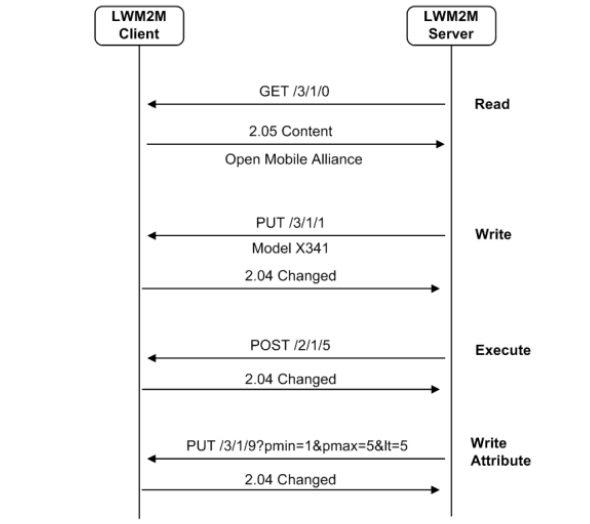
\includegraphics[scale=0.65]{images/lwm2m/command_diagram.png}
\caption{LwM2M Device Access\cite{LwM2MInterfaces}}
\end{figure}
In der Grafik sieht man drei Beispielanfragen eines LwM2M-Servers.

Die erste Anfrage ist ein Read-Request. Der Server sendet ein GET auf die gewünschte Ressource, in diesem Beispiel ist dies 3/1/0 und wartet auf den Response. Der Client überprüft nun seine ACLs und wenn der Server berechtigt ist, sendet der Client ein Response  mit den Content zurück. Wenn die Ressource nicht vorhanden oder der Server nicht berechtigt ist, erhält der Server einen anderen Response als Content. Dies könnte zum Beispiel ''Not Found'' sein, falls die Ressource nicht vorhanden ist.

Der Write-Request ist sehr ähnlich aufgebaut. Anstelle eines GET-Requests sendet der Server ein PUT-Request. In diesem Request wird wieder die gewünschte Ressource-URL angesprochen und die zu schreibenden Daten werden direkt mit dem Request mitgesendet. Hier gibt der Client wieder mit ''Changed'' Antwort, falls alles in Ordnung ist.

Auch der Execute funktioniert gleich wie die anderen zwei Requests. Anstelle von GET oder PUT wird hier ein POST verwendet. Die Antwort beinhaltet wie beim Write-Requests ein ''Changed'' Status, damit der Server weiss, dass alles funktioniert hat.

\newpage

\subsubsection{Reporting - Allgemein}
LwM2M bietet neben den von Hand ausgeführten Read auch ein Observer an. Dieser wird mit dem Reporting Interface beschrieben. Reporting bietet dabei drei Funktionen. Observe, Notify und Cancel Observation. Mit dem Observe Befehl meldet sich ein Server beim Client und meldet sich an. Bei jeder Zustandsänderung der Ressource meldet sich der Client beim Server und sendet die neuen Daten an diesen Der Server kann so stetig wechselnde Daten sehr einfach überwachen, ohne die Ressource jedes mal von Hand upzudaten.
\subsubsection{Reporting - Ablauf}
Im Grunde wird hier ein normales Observer-Pattern umgesetzt. Der Server ist der Observer und der Client ist das Subject. Initiiert wird dieser Vorgang immer vom Server aus. 
\begin{figure}[H]
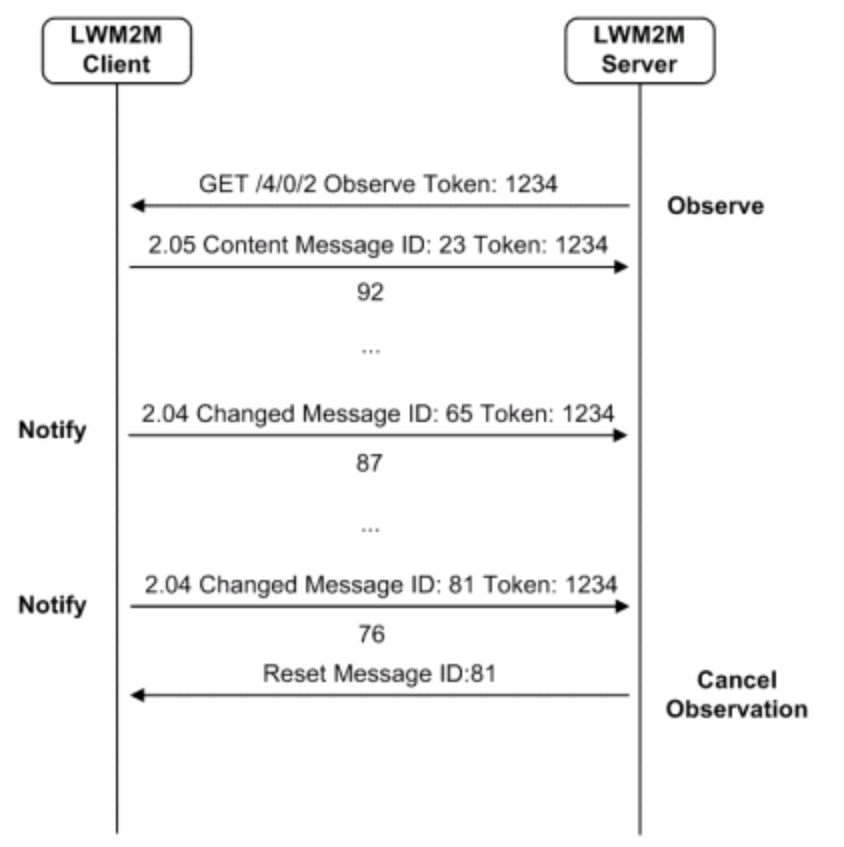
\includegraphics[scale=0.4]{images/lwm2m/report_diagram.png}
\caption{LwM2M Reporting\cite{LwM2MInterfaces}}
\end{figure}
Um eine Ressource zu Überwachen, sendet der Server ein GET-Request an die gewünschte Ressource-URL mit einem Observe Token. Direkt nach dem Anmelden des Observers meldet der Client den aktuellen Wert der Ressource mit einer Content Message ID und dem Observer Token.

Bei jeder Änderung der Ressource erstellt der Client wieder ein neuer Response mit einer Changed Message ID und dem Token und sendet diese an alle Observer zurück.

Möchte der Server die Ressource nicht länger Überwachen, sendet der Server ein Reset zurück. Dieser Reset beinhaltet die letzte Changed Message ID. Hier im Beispiel sieht man dies ganz am Schluss der Grafik. So meldet sich der Server ab und erhält keine weiteren Notifikationen.

\subsection{Fazit}